% Created by tikzDevice version 0.12 on 2019-02-08 11:09:30
% !TEX encoding = UTF-8 Unicode
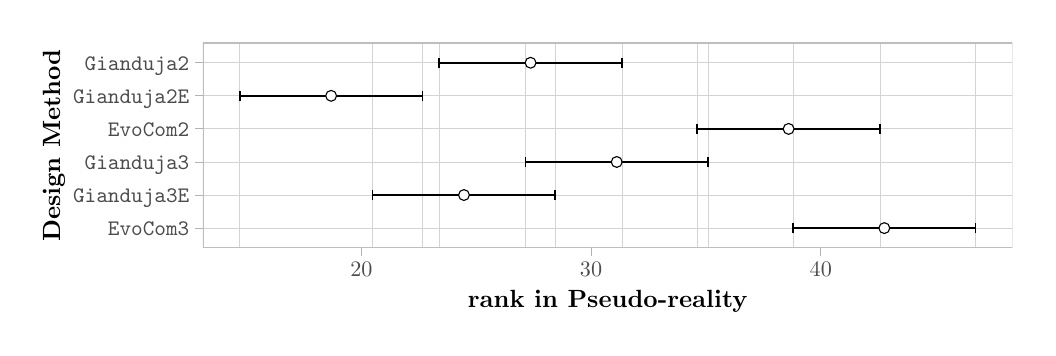
\begin{tikzpicture}[x=1pt,y=1pt]
\definecolor{fillColor}{RGB}{255,255,255}
\path[use as bounding box,fill=fillColor,fill opacity=0.00] (0,0) rectangle (361.35,108.41);
\begin{scope}
\path[clip] (  0.00,  0.00) rectangle (361.35,108.40);
\definecolor{drawColor}{RGB}{255,255,255}
\definecolor{fillColor}{RGB}{255,255,255}

\path[draw=drawColor,line width= 0.6pt,line join=round,line cap=round,fill=fillColor] (  0.00,  0.00) rectangle (361.35,108.40);
\end{scope}
\begin{scope}
\path[clip] ( 63.34, 28.81) rectangle (355.85,102.90);
\definecolor{fillColor}{RGB}{255,255,255}

\path[fill=fillColor] ( 63.34, 28.81) rectangle (355.85,102.90);
\definecolor{drawColor}{RGB}{211,211,211}

\path[draw=drawColor,line width= 0.3pt,line join=round] ( 63.34, 71.83) --
	(355.85, 71.83);

\path[draw=drawColor,line width= 0.3pt,line join=round] ( 63.34, 35.98) --
	(355.85, 35.98);

\path[draw=drawColor,line width= 0.3pt,line join=round] ( 63.34, 95.73) --
	(355.85, 95.73);

\path[draw=drawColor,line width= 0.3pt,line join=round] ( 63.34, 83.78) --
	(355.85, 83.78);

\path[draw=drawColor,line width= 0.3pt,line join=round] ( 63.34, 59.88) --
	(355.85, 59.88);

\path[draw=drawColor,line width= 0.3pt,line join=round] ( 63.34, 47.93) --
	(355.85, 47.93);

\path[draw=drawColor,line width= 0.2pt,line join=round] (307.97, 28.81) -- (307.97,102.90);

\path[draw=drawColor,line width= 0.2pt,line join=round] (214.73, 28.81) -- (214.73,102.90);

\path[draw=drawColor,line width= 0.2pt,line join=round] (142.65, 28.81) -- (142.65,102.90);

\path[draw=drawColor,line width= 0.2pt,line join=round] (342.55, 28.81) -- (342.55,102.90);

\path[draw=drawColor,line width= 0.2pt,line join=round] (245.86, 28.81) -- (245.86,102.90);

\path[draw=drawColor,line width= 0.2pt,line join=round] (190.66, 28.81) -- (190.66,102.90);

\path[draw=drawColor,line width= 0.2pt,line join=round] (241.96, 28.81) -- (241.96,102.90);

\path[draw=drawColor,line width= 0.2pt,line join=round] (148.72, 28.81) -- (148.72,102.90);

\path[draw=drawColor,line width= 0.2pt,line join=round] ( 76.64, 28.81) -- ( 76.64,102.90);

\path[draw=drawColor,line width= 0.2pt,line join=round] (276.54, 28.81) -- (276.54,102.90);

\path[draw=drawColor,line width= 0.2pt,line join=round] (179.84, 28.81) -- (179.84,102.90);

\path[draw=drawColor,line width= 0.2pt,line join=round] (124.64, 28.81) -- (124.64,102.90);
\definecolor{drawColor}{RGB}{0,0,0}

\path[draw=drawColor,line width= 0.6pt,line join=round] (307.97, 70.04) --
	(307.97, 73.62);

\path[draw=drawColor,line width= 0.6pt,line join=round] (307.97, 71.83) --
	(241.96, 71.83);

\path[draw=drawColor,line width= 0.6pt,line join=round] (241.96, 70.04) --
	(241.96, 73.62);

\path[draw=drawColor,line width= 0.6pt,line join=round] (214.73, 93.94) --
	(214.73, 97.53);

\path[draw=drawColor,line width= 0.6pt,line join=round] (214.73, 95.73) --
	(148.72, 95.73);

\path[draw=drawColor,line width= 0.6pt,line join=round] (148.72, 93.94) --
	(148.72, 97.53);

\path[draw=drawColor,line width= 0.6pt,line join=round] (142.65, 81.99) --
	(142.65, 85.58);

\path[draw=drawColor,line width= 0.6pt,line join=round] (142.65, 83.78) --
	( 76.64, 83.78);

\path[draw=drawColor,line width= 0.6pt,line join=round] ( 76.64, 81.99) --
	( 76.64, 85.58);

\path[draw=drawColor,line width= 0.6pt,line join=round] (342.55, 34.19) --
	(342.55, 37.77);

\path[draw=drawColor,line width= 0.6pt,line join=round] (342.55, 35.98) --
	(276.54, 35.98);

\path[draw=drawColor,line width= 0.6pt,line join=round] (276.54, 34.19) --
	(276.54, 37.77);

\path[draw=drawColor,line width= 0.6pt,line join=round] (245.86, 58.09) --
	(245.86, 61.67);

\path[draw=drawColor,line width= 0.6pt,line join=round] (245.86, 59.88) --
	(179.84, 59.88);

\path[draw=drawColor,line width= 0.6pt,line join=round] (179.84, 58.09) --
	(179.84, 61.67);

\path[draw=drawColor,line width= 0.6pt,line join=round] (190.66, 46.14) --
	(190.66, 49.72);

\path[draw=drawColor,line width= 0.6pt,line join=round] (190.66, 47.93) --
	(124.64, 47.93);

\path[draw=drawColor,line width= 0.6pt,line join=round] (124.64, 46.14) --
	(124.64, 49.72);

\path[draw=drawColor,line width= 0.4pt,line join=round,line cap=round,fill=fillColor] (274.96, 71.83) circle (  1.96);

\path[draw=drawColor,line width= 0.4pt,line join=round,line cap=round,fill=fillColor] (181.72, 95.73) circle (  1.96);

\path[draw=drawColor,line width= 0.4pt,line join=round,line cap=round,fill=fillColor] (109.65, 83.78) circle (  1.96);

\path[draw=drawColor,line width= 0.4pt,line join=round,line cap=round,fill=fillColor] (309.55, 35.98) circle (  1.96);

\path[draw=drawColor,line width= 0.4pt,line join=round,line cap=round,fill=fillColor] (212.85, 59.88) circle (  1.96);

\path[draw=drawColor,line width= 0.4pt,line join=round,line cap=round,fill=fillColor] (157.65, 47.93) circle (  1.96);
\definecolor{drawColor}{RGB}{190,190,190}

\path[draw=drawColor,line width= 0.6pt,line join=round,line cap=round] ( 63.34, 28.81) rectangle (355.85,102.90);
\end{scope}
\begin{scope}
\path[clip] (  0.00,  0.00) rectangle (361.35,108.41);
\definecolor{drawColor}{gray}{0.30}

\node[text=drawColor,anchor=base east,inner sep=0pt, outer sep=0pt, scale=  0.80] at ( 58.39, 69.08) {\texttt{EvoCom2}};

\node[text=drawColor,anchor=base east,inner sep=0pt, outer sep=0pt, scale=  0.80] at ( 58.39, 33.22) {\texttt{EvoCom3}};

\node[text=drawColor,anchor=base east,inner sep=0pt, outer sep=0pt, scale=  0.80] at ( 58.39, 92.98) {\texttt{Gianduja2}};

\node[text=drawColor,anchor=base east,inner sep=0pt, outer sep=0pt, scale=  0.80] at ( 58.39, 81.03) {\texttt{Gianduja2E}};

\node[text=drawColor,anchor=base east,inner sep=0pt, outer sep=0pt, scale=  0.80] at ( 58.39, 57.13) {\texttt{Gianduja3}};

\node[text=drawColor,anchor=base east,inner sep=0pt, outer sep=0pt, scale=  0.80] at ( 58.39, 45.18) {\texttt{Gianduja3E}};
\end{scope}
\begin{scope}
\path[clip] (  0.00,  0.00) rectangle (361.35,108.41);
\definecolor{drawColor}{gray}{0.70}

\path[draw=drawColor,line width= 0.3pt,line join=round] ( 60.59, 71.83) --
	( 63.34, 71.83);

\path[draw=drawColor,line width= 0.3pt,line join=round] ( 60.59, 35.98) --
	( 63.34, 35.98);

\path[draw=drawColor,line width= 0.3pt,line join=round] ( 60.59, 95.73) --
	( 63.34, 95.73);

\path[draw=drawColor,line width= 0.3pt,line join=round] ( 60.59, 83.78) --
	( 63.34, 83.78);

\path[draw=drawColor,line width= 0.3pt,line join=round] ( 60.59, 59.88) --
	( 63.34, 59.88);

\path[draw=drawColor,line width= 0.3pt,line join=round] ( 60.59, 47.93) --
	( 63.34, 47.93);
\end{scope}
\begin{scope}
\path[clip] (  0.00,  0.00) rectangle (361.35,108.41);
\definecolor{drawColor}{gray}{0.70}

\path[draw=drawColor,line width= 0.3pt,line join=round] (120.58, 26.06) --
	(120.58, 28.81);

\path[draw=drawColor,line width= 0.3pt,line join=round] (203.58, 26.06) --
	(203.58, 28.81);

\path[draw=drawColor,line width= 0.3pt,line join=round] (286.58, 26.06) --
	(286.58, 28.81);
\end{scope}
\begin{scope}
\path[clip] (  0.00,  0.00) rectangle (361.35,108.41);
\definecolor{drawColor}{gray}{0.30}

\node[text=drawColor,anchor=base,inner sep=0pt, outer sep=0pt, scale=  0.80] at (120.58, 18.35) {20};

\node[text=drawColor,anchor=base,inner sep=0pt, outer sep=0pt, scale=  0.80] at (203.58, 18.35) {30};

\node[text=drawColor,anchor=base,inner sep=0pt, outer sep=0pt, scale=  0.80] at (286.58, 18.35) {40};
\end{scope}
\begin{scope}
\path[clip] (  0.00,  0.00) rectangle (361.35,108.41);
\definecolor{drawColor}{RGB}{0,0,0}

\node[text=drawColor,anchor=base,inner sep=0pt, outer sep=0pt, scale=  0.90] at (209.60,  7.44) {\bfseries rank in Pseudo-reality};
\end{scope}
\begin{scope}
\path[clip] (  0.00,  0.00) rectangle (361.35,108.41);
\definecolor{drawColor}{RGB}{0,0,0}

\node[text=drawColor,rotate= 90.00,anchor=base,inner sep=0pt, outer sep=0pt, scale=  0.90] at ( 11.71, 65.86) {\bfseries Design Method};
\end{scope}
\end{tikzpicture}
